
\sectionOne{Introduction}
% Paragraph about how our society relates to combustion

Combustion has played a crucial role in society for a long time and in many aspects.
It is the driving force behind transportation which is critical to the world economy and supply chain.
While it is necessary, transportation accounts for substantial amounts of greenhouse gas emissions which can adversely affect the environment and public health \cite{van_fan_review_2018, manisalidis_environmental_2020}.
Combustion is also a driving force behind wildfire which likewise produces emissions that negatively impact the environment and public health.
Wildfire is particularly impactful with yearly averages of 70,600 wildfires and 7.0 million acres burned since 2000 \cite{hoover_wildfire_2021}.
The emissions produced, regardless of their source, are complicated and composed of many different chemical species which contribute to secondary pollutants such as carbon monoxide (CO), volatile organic compounds (VOCs), sulphur oxide (SOx), and nitrogen oxide (NOx) \cite{van_fan_review_2018}.

% Paragraph about challenges and modeling needs
Mitigation of these emissions and their impacts requires that we continue to develop understanding of them which is not without challenges.
Specifically, modeling on practical scales can be challenging due to large computational expense associated with detailed chemistry.
There are methods that reduce this expense by sacrificing detail such as hybrid chemistry, analytically reduced chemistry, and multicomponent surrogates \cite{felden_including_2016}.
However, in doing so, we cannot adequately model the impact or behavior of fuels or byproducts that require a large number of species.

% Paragraph about what current software has achieved
Real fuel chemistry remains out of reach because of the computational demand associated with a large kinetic mechanisms, i.e., a large number of species and reactions involved.
Current software such as GEOS-chem has achieved global atmospheric chemistry modeling with a couple hundred species by implementing the use of parallel systems \cite{eastham_geos-chem_2018}.
However, models of SOAs have resulted in chemical mechanisms in excess of 5000 species \cite{li_modeling_2015}.
Modeling of complicated fuels to determine accurate emissions also requires a large numbers of species, e.g., a detailed mechanism by Sarathy et al. modeling 2-methylalkanes from C7 to C20 contains nearly 7200 species \cite{sarathy_comprehensive_2011}.

% Paragraph about needed research
According to the CFD 2030 Vision report, further research is needed to accelerate chemical kinetics solutions so that CFD simulations are not bottlenecked by the chemistry \cite{slotnick_cfd_2014}.
The inclusion of chemistry in LES simulations currently relies on methods that reduce the size of the mechanism such as hybrid chemistry, analytically reduced chemistry, and multicomponent surrogates \cite{felden_including_2016}.
However, if we want to approach "real fuel" chemistry, these methods are not viable and further investigation into the current solutions of these systems of equations is required.
These systems are numerically stiff and require implicit integration which is particularly expensive because it requires the inversion of large matrices (the number of species squared).
Direct solution methods to the linear systems using the most simplistic inversion techniques like Gauss–Jordan elimination can be incredibly expensive with a complexity up to $\mathcal{O}(n^3)$.
Despite improvements of such techniques, the bottleneck still exists and requires further research into accelerating the chemical kinetics.

% Paragraph about our study
This study strives toward improving our modeling capabilities of large kinetic mechanisms by leveraging preconditioning and sparse matrix solvers.
To achieve this, we have extended our github fork of \cantera{}\footnote{https://github.com/anthony-walker/cantera} to include preconditioning functionality and specifically the adaptive preconditioning technique as described by McNenly et al. \cite{mcnenly_faster_2015}.
This study specifically focuses on applying this technique to ideal gas constant pressure systems in the hopes of obtaining substantial speed-up.
We first discuss related work and distinguish our work from prior studies in section \ref{p1:related-section}. Next, we describe objectives, methods, study
parameters, and tests in section \ref{p1:methods-section}. As expected, this is followed
with results, discussion, and conclusions.

\sectionOne{Related Work}
\label{p1:related-section}

Accelerating the simulation of large chemical kinetics mechanisms has been approached in many different ways because several steps in the solution process is rather involved.
Specifically, we use a backward differentiation formula (BDF) that is part of the \sundials{} \cvodes{} package \cite{cohen_cvode_1996, hindmarsh_sundials_2005}.
The BDF method in \cvodes{} relies on Newton-Iterations as the nonlinear solver which requires several linear iterations per nonlinear step.
We use a Left Preconditioned Generalized Minimum Residual method for the linear iterations which solves a preconditioned system.
The solution of the preconditioned system is determined via an incomplete LU decomposition.

%Paragraph about preconditioner specifics
The type of preconditioning used is referred to as Adaptive Preconditioning and was originally developed with constant volume systems by McNenly et al. \cite{mcnenly_faster_2015}.
It is a Jacobian based preconditioner that makes several simplifications to accelerate its formulation.
In regards to species rate derivatives, Adaptive preconditioning neglects thirdbody efficiencies and pressure dependence in the determination of species related elements.
It also uses finite difference approximations for derivatives with respect to temperature and prunes non-diagonal values below a specified threshold.
This pruning is intended improve the benefit of leveraging sparse solvers by removing elements.

There have been several approachs with the goal of accelerating the integration of chemical kinetics in similar ways.
A common theme amongst these approaches is that taking advantage of the sparsity of the system is often the best way forward.
The most similar approaches focus on the linear solver and applying different techniques or integrators to the integration \cite{liang_towards_2009, mcnenly_faster_2015, perini_study_2014, anzt_preconditioned_2017}.
Many other approaches rely on the sparsity as well but focus on the methods used to form the Jacobian.
The use analytical, semi-analytical, and approxmiate Jacobians is popular amongst these methods \cite{perini_analytical_2012,  dijkmans_gpu_2014, niemeyer_initial_2015, niemeyer_pyjac_2017, lapointe_sparse_2019, lapointe_computationally-efficient_2020}.
Alternatively, a Jacobian free method has also been implemented \cite{morii_erena_2016}.

There have also been approachs adjacently related that are not a fully implicit or traditional means of solving chemical kinetics
For example, explicit methods and on differing hardware such as GPUS have been explored \cite{niemeyer_accelerating_2014, curtis_investigation_2017}.
Likewise, GPUs have been used for developement of an analytical Jacobian and preconditioned Krylov solvers \cite{dijkmans_gpu_2014,anzt_preconditioned_2017}.
Semi-implicit methods that treat stiff species implicitly have been implemented \cite{gao_dynamic_2015, xu_sparse_2016, savard_computationally-efficient_2015}.
Finally, DAEPACK is an auto-differentiation approach to accelerate kinetics \cite{schwer_upgrading_2002}.

In summary, there are many approaches that have been implemented to accelerate chemical kinetics.
Many of these approaches leverage a sparse solver, similar to this work.
The primary difference between our work and other stuides is our focus on a semi-analytical approximate Jacobian which is used as the basis for a preconditioner.
More specifically, the way the preconditioner is formed and the assumptions applied separates it from other preconditioner studies.
The closest study is this work's predecessor by McNenly et al. \cite{mcnenly_faster_2015}.
We differ from this study by applying the technique to a different system---an ideal gas constant pressure plug flow reactor.

Consequently, our goals for this study are as follows:
\begin{itemize}
    \item Apply adaptive preconditioning to a constant pressure system and assess potential differences in applying the preconditioner to a new system.
    \item Determine the impact of the threshold on the preconditioner and provide recommendations or heuristics.
    \item Determine the role of any assumptions and methods in any performance increase.
    \item Provide recommendations for future work.
\end{itemize}


\sectionOne{Methods}
\label{p1:methods-section}
Adaptive preconditioning is the focus of our work but review of
the other components is necessary for a complete understanding of how
our work contributes and fits within the numerics.
We implemented adaptive preconditioning to integrate a constant pressure ideal gas plug flow reactor.
We ran each test case 100 times and used average values to help account for any unknown variability in timing the runs.
In this problem, we provide a stoichiometric fuel air mixture at atmospheric pressure and an initial temperature of $1500\,K$.
We selected these initial conditions to produce an ignition event and integrated to a time of one second.
We integrated this problem with a range of preconditioner thresholds from $10^{-18}$ to $10^{-1}$ and 0.
We also spanned range of mechanisms providing a species from 10 to 7171---all of which are listed succinctly in Table~\ref{t1:mechanisms}.

First we set up the system for our PFR by defining a state vector of length $\ell$.
\begin{equation}
    \ell = \nspecies + 1,
\end{equation}
where $\nspecies$ is the number of chemical species.
We represent this system with the state vector,
\begin{equation}
    \S{} = \{T, n_1, n_2, n_3, \cdots, n_{\nspecies}\},\quad\S{}\in\mathbb{R}^\ell
\end{equation}
where $T$ is temperature and $n_i$ is the moles of species $i$.
We then defined our system of ODEs as
\begin{equation}
    \label{eq:ode-system}
    \frac{d\S{}}{dt} = \F{t,\S{}}
\end{equation}
where $\F{t,\S{}}$ can be a nonlinear function of $\S{}$ and $t$.

The integration of Eq.~\eqref{eq:ode-system} is composed of several steps that are highlighted in Figure~\ref{f:integration_process}.
The process starts by setting up the preconditioner if necessary.
The nonlinear solver then starts to make iterations which requires iterations of the linear solver.
In some cases, the preconditioner will need to be reformed during the nonlinear iterations and this is done as is necessary.
Consequently, we discuss the different steps of a time step in the same order.

\begin{figure}[h!]
    \centering
    \IntegrationOverview[0.85]{}
    \caption{General procedure of the of a time step.}
    \label{f:integration_process}
\end{figure}

\sectionTwo{Adaptive Preconditioning Setup}
\label{sec:methods-adaptive}
Adaptive preconditioning originally applied to constant volume systems
by McNenly et al.\cite{mcnenly_faster_2015} works by using an
approximate or skeletal version of the Jacobian.
The original authors used a mass fraction Jacobian but this method results in a fully dense Jacobian for constant pressure systems.
So, we use a mole based Jacobian, $\J{\S{}}$, to develop the preconditioner, $\AP$.
This skeletal version is developed by eliminating elements below a certain threshold, computing some numerical derivatives, and neglecting thirdbody efficiency and pressure dependence in the analytical derivatives $\frac{\partial \dot{n}_i}{\partial n_j}$.
The skeletal Jacobian used in this work can be calculated as
\begin{equation}
    \J{\S{}} =
    \begin{bmatrix}
        \jacline{\dot{T}}
        \jacline{\dot{n}_{1}}
        \dotsline{}
        \jacline{\dot{n}_{\nspecies}}
    \end{bmatrix},
\end{equation}
where $\dot{n}_i$ is the net rate of production of species $n_i$ in moles.
Similarly, $\dot{\omega}_i$ is the net rate of species production in concentration.

%
% ----------------d(n_j)/dT------------------
%
We first consider the derivatives with respect to temperature that are found by finite difference. We generalize them as $\frac{\partial \dot{\eta}}{\partial T}$ where $\eta$ is any state variable and $\epsilon$ is a perturbation---machine precision.
This gives
\begin{equation}
    \label{eq:temp-dervs}
    \frac{\partial \dot{\eta}}{\partial T} = \frac{\dot{\eta}\big\vert_{\epsilon+T}-\dot{\eta}\big\vert_{T}}{T\sqrt{\epsilon}}.
\end{equation}

%
% ----------------d(omega_dot)/dn_j------------------
%
The species production derivatives, $\frac{\partial \dot{n}_i}{\partial n_j}$, require looping over the species and reactions where $\nreactions$ is the total number of reactions.
These derivatives are intuitive in terms of concentration but the current preconditioner is based in moles so a conversion of some derivatives is necessary and can be found as
\begin{align}
    \conc{n_j} &= \frac{n_j}{V}\\
    \frac{\partial \conc{n_j}}{\partial n_j} &= \frac{1}{V},
\end{align}
where $V$ is the volume of the system.
The species to species derivatives used in the preconditioner can then be found as
\begin{equation}
    \frac{\partial \dot{n}_i}{\partial n_j} = \frac{\partial V}{\partial n_j} \omega_i + V\frac{\partial \dot{\omega}}{\partial n_j}
\end{equation}
It is easiest to breakdown the former equation into components to determine the overall terms in a piecewise manner.
So, we first consider the derivative of the ratelaw with respect to moles.
\begin{multline}
    \label{eq:full-spec-spec}
    V \frac{\partial \dot{\omega}_i}{\partial n_j} = V \frac{\partial \dot{\omega}_i}{\partial \conc{n_j}} \frac{\partial \conc{n_j}}{\partial n_j} \\ = \ReacSum{\nu_{i,k}b_k\frac{\partial R_k}{\partial \conc{n_j}} + \nu_{i,k}R_k\frac{\partial b_k}{\partial\conc{n_j}}},
\end{multline}
where $b_k=1$ which discards the thirdbody portion of the rate law and the volume terms cancel.
Eq.~\eqref{eq:full-spec-spec} then simplfies to
\begin{equation}
    \label{eq:spec-spec-derv}
    \frac{\partial \dot{\omega}_i}{\partial n_j} = \ReacSum{\nu_{i,k}\frac{\partial R_k}{\partial \conc{n_j}}}.
\end{equation}
The rate of progress derivative is consequently broken down into $\frac{\partial R_k}{\partial\conc{n_j}}$ is the rate of progress derivative
\begin{multline}
    \frac{\partial R_k}{\partial\conc{n_j}} = k_{f,k}{v_{k,j}^\prime} \conc{n_j}^{v_{k,j}^\prime-1}\ReactSpecProd{\conc{n_h}^{v_{k,h}^\prime}}\\
    -k_{r,k}v_{k,j}^{\prime\prime}\conc{n_j}^{v_{k,j}^{\prime\prime}-1}\ProdSpecProd{\conc{n_h}^{v_{k,h}^{\prime\prime}}}
\end{multline}
where $\nu$ is the stoichiometric coefficient, $k$ is the reaction rate, $\alpha$ and $\beta$ represent reactant and product species for the reaction.
The next term we need to determine is $\frac{\partial V}{\partial n_j} \omega_i$.
We start with the ideal gas law in the form
\begin{equation}
     V = \frac{NRT}{P}.
\end{equation}
We use this relation and simplify the equation to obtain
\begin{equation}
    \frac{\partial V}{\partial n_j} = \frac{\partial V}{\partial N}\frac{\partial N}{\partial n_j} = \frac{RT}{P} = \frac{V}{N}.
\end{equation}
The final expression is then
\begin{multline}
    \frac{\partial \dot{n}_i}{\partial n_j} = \frac{V}{N} \omega_i + \\
    \ReacSum{\nu_{i,k} k_{f,k}{v_{k,j}^\prime} \conc{n_j}^{v_{k,j}^\prime-1}\ReactSpecProd{\conc{n_h}^{v_{k,h}^\prime}}} + \\
    \ReacSum{-\nu_{i,k} k_{r,k}v_{k,j}^{\prime\prime}\conc{n_j}^{v_{k,j}^{\prime\prime}-1}\ProdSpecProd{\conc{n_h}^{v_{k,h}^{\prime\prime}}}}.
\end{multline}
%
% ----------------d(dT/dt)/dn_j------------------
%
Next, we consider the derivatives of temperature with respect to different species.
The derivatives, $\frac{\partial\dot{T}}{\partial n_j}$, are found by considering the energy equation as
\begin{equation}
    \frac{\partial T}{\partial t} = \frac{a}{b} = \frac{-\SpecSum{\bar{h}_k\dot{\omega}_k}}{\SpecSum{\conc{n_k} \hat{c}_{p,k}}} = \frac{-V\SpecSum{\bar{h}_k\dot{n}_k}}{V \SpecSum{n_k \hat{c}_{p,k}}},
\end{equation}
where $\hat{c}_{p,k}$ and $\bar{h}_k$ are the molar constant pressure specific heat and enthalpy of species $n_k$, respectively.
The initial equation is concentration based but again we are using moles so we adjust the equation to account for that.
We find the derivatives by first applying the quotient rule
\begin{equation}
    \frac{\partial \dot{T}}{\partial n_j} = \frac{ab^\prime-a^\prime b}{b^2}.
\end{equation}
We broke this into parts  to simplify the process.
So, we find the appropriate terms for each of the needed derivatives and then cancel terms where possible.
The first term is found as
\begin{equation}
    a^\prime b = -N\hat{c}_p\SpecSum{\bar{h}_k \frac{\partial \dot{n}_k}{\partial n_j}}
\end{equation}
where the contained partial derivatives are actually other Jacobian elements.
This is convenient because we can first find those elements and then reuse them.
We assume that $c_{p,j}$ is constant with respect to other species because it is an ideal gas which gives
\begin{equation}
    a b^\prime = -c_{p,j}\SpecSum{\bar{h}_k \dot{n}_k}.
\end{equation}
Finally, we combine the two part into the generalized temperature derivative with respect to a species $j$,
\begin{equation}
    \label{eq:temp-species}
    \frac{\partial \dot{T}}{\partial n_j} = \frac{-N\hat{c}_p\SpecSum{\bar{h}_k \frac{\partial \dot{n}_k}{\partial n_j}} + c_{p,j}\SpecSum{\bar{h}_k \dot{n}_k}}{(N\hat{c}_p)^2}.
\end{equation}

The final step in $\AP$ formation is then removing non-diagonal elements below a threshold value, $\xi$, as
\begin{equation}
    \AP[i,j] =
    \begin{cases}
        0 & \J{\S{}}[i,j] < \xi \text{ and } i \neq j, \\
        \J{\S{}}[i,j] & i = j,
    \end{cases}
\end{equation}
We can now form the preconditioner and begin the integration.

\sectionTwo{Newton Iteration}
The nonlinear portion of the integration is performed with Newton's method
which is a linear approximation to the nonlinear system using
a Taylor series expansion.
\sundials{} does this internally, however, discussion is useful to understand where the preconditioner is used during the integration \cite{hindmarsh_sundials_2005}.
We start this process by discretizing Equation~\eqref{eq:ode-system} with a general, variable order, backward differentiation formula (BDF) as
\begin{equation}
    \sum^{\Omega}_{i=0}{\alpha^{n-i} \S{}^{n-i}} = \beta \Delta t\F{t, \S{}_{n}}
\end{equation}
where $\Omega$ is the order, $n$ is the current time step, and
$\alpha^{k}$ and $\beta$ are coefficients used to achieve the order.
For example, in the case of backward Euler (first order BDF), $\Omega = 1$, $\alpha_0
= 1$, $\alpha_1 = -1$, and $\beta = 1$.
We then put the formula in the form
\begin{equation}
    \sum^{\Omega}_{i=0}{\alpha^{n-i} \S{}^{n-i}} - \beta \Delta t\F{t, \S{}^{n}} = 0
\end{equation}
which is a system of nonlinear algebraic equations.
We define this system as
\begin{equation}
    \N{\S{}_n} \equiv \sum^{\Omega}_{i=0}{\alpha^{n-i} \S{}^{n-i}} - \beta \Delta t\F{t, \S{}^{n}} = 0.
\end{equation}
The Taylor series approximation $\N{\S{}^{n}}$ is then
\begin{multline}
    \label{p1:eq:taylor_series}
    \N{\S{}^{}} = \N{\S^{n-1}} + \J{\N{\S{}^{n-1}}}(\S{}^{n}-\S{}^{n-1}) \\ + \text{higher order terms} = 0.
\end{multline}
We truncate the series \eqref{p1:eq:taylor_series} after the linear term
to provide the linear system of equations with iteration index $k$ as
\begin{equation}
     \J{\N{\S{}^{k}}}(\S{}^{k+1}-\S{}^{k}) = -\N{\S^{k}},\quad k\in\mathbb{R}^{+}_{0}
\end{equation}
which is iterated until it converges to the solution to the nonlinear system of
equations for time step $n$.
This formula is solved for future iterates with a few manipulations.
The Jacobian of $\N{\S{}^{k}}$ can be simplied to
\begin{equation}
    \K{\S{}^{k}} \equiv \J{\N{\S{}^{k}}} = I-\Delta t \beta\J{\F{t,\S{}^{k}}}
\end{equation}
which we substitute into the former equation to yield
\begin{equation}
    \K{\S{}^{k}}(\S{}^{k+1}-\S{}^{k}) = -\N{\S^{k}}.
\end{equation}
We then form our iteration formula as
\begin{equation}
    \label{eq:newIterForm}
    \S{}^{k+1} = \S{}^{k}-\big[\K{\S{}^{k}}\big]^{-1}\N{\S{}^{k}}.
\end{equation}
Now that we have the iteration formula for approximating the nonlinear steps, we can dive into the details of the linear solver.

\sectionTwo{Preconditioned GMRES}
The nonlinear solution requires several linear iterations to complete a nonlinear iteration.
In this work, we use a left preconditioned GMRES method to leverage sparsity of large kinetic mechanisms.
We consider the system
\begin{equation}
    \label{sys:axb}
    A x = b,\quad A\in \mathbb{C}^{m\times n},\, m\geq n ,\,b\in \mathbb{C}^{m}
\end{equation}
to describe preconditioning and \gmres{}.
A direct solution of
\eqref{sys:axb} would be
\begin{equation}
    x = A^{-1}b.
\end{equation}
However, when the problem is ill-posed it helps to precondition the
system as
\begin{equation}
    \AP{}^{-1}Ax = \AP{}^{-1}b.
\end{equation}
Ideally, the preconditioner, $\AP{}$, will be close to $A$ and
well-posed so convergence to the solution is accelerated. If $\AP{}=A$
then the solution would be obtained exactly from preconditioning.
Applying preconditioning to \gmres{}, we define the residual $\delta$.
\begin{equation}
    \delta = ||\AP{}^{-1}b-\AP{}^{-1}Ax||_2
\end{equation}
and attempt to find $x$ such that $\delta$ is minimized.
Translating this idea, we put our system in the form
\begin{equation}
    \K{\S{}^{k}}\S{}^{k+1} =  \K{\S{}^{k}}\S{}^{k}-\N{\S^{k}}
\end{equation}
and define the right hand side as $\R{\S{}^{k}}$ to get
\begin{equation}
    \label{eq:mf-system}
    \K{\S{}^{k}}\S{}^{k+1} = \R{\S{}^{k}}.
\end{equation}
Applying the preconditioner to the system, we obtain
\begin{equation}
    \MP{\S{}^{k}}^{-1}\K{\S{}^{k}}\S{}^{k+1} = \MP{\S{}^{k}}^{-1}\R{\S{}^{k}}
\end{equation}
which can be back substituted to form a final expression for the residual.


We applied the preconditioned \gmres{} with \sundials{} by a user-defined function, \psolve{}, which requires that the user solve the system
\begin{equation}
    \AP{}z = r
\end{equation}
where $r$ in this case is equivalent to $b-Ax$.
The result is the preconditioned residual in the output vector $z$ as
\begin{equation}
    z =\AP{}^{-1}(b-Ax).
\end{equation}
Here, we apply the incomplete LU decomposition from the Eigen C++ package to determine the solution to the former system \cite{guennebaud_eigen_2010}.
The 2-norm of $z$ is then the residual $\delta$.
Applying the \sundials{} method to our system, we obtain
\begin{equation}
    z = \MP{\S^{k}}^{-1}\big[\R{\S{}^{k}}-\K{\S{}^{k}}\S{}^{k+1}\big] = \MP{\S^{k}}^{-1}\B{\S{}^{k}}
\end{equation}
where the preconditioner is formed with adaptive preconditioning described in Section~\ref{sec:methods-adaptive}.

To summarize the integration, we apply adaptive preconditioning to a constant pressure ideal gas plug flow reactor.
The integration is an implict BDF formulation that uses Newton iterations for the nonlinear solution and preconditioned \gmres{} for the linear solution.
The preconditioned solution used by \gmres{} is formed with an incomplete LU factorization.
These methods are implemented within \cantera{} and take advantage of \sundials{}\cite{hindmarsh_sundials_2005} and \eigen{}\cite{guennebaud_eigen_2010}.


\sectionOne{Results}

As a reminder, we applied adaptive preconditioning to an ideal gas constant pressure plug flow reactor with an ignition event.
We implemented this work inside of the open source package, \cantera{}, and compared the results to the traditional direct dense solver.
We applied a threshold range of $10^{-18}$ to $10^{-1}$ and $0$.
We analyzed all of the species listed in Table~\ref{t1:mechanisms} which provide a species range of 10-7171.
Here, we report the average values of 100 runs of each test case.

First, we consider the best case scenario speed up.

\begin{table*}[ht] \small
    \centering
    \begin{tabular}{|lcccc|}
        \hline
        Mechanism & Formula & Species & Reactions & Optimal Threshold ($\xi$)\\
        \hline
        Hydrogen\cite{smith_gri-mech_1999} & \ce{H2} & 10 & 29 & 0 \\
        GRI Mech\cite{smith_gri-mech_1999} & \ce{CH4} & 55 & 325 & 0 \\
        DME-Propane\cite{dames_detailed_2016} & \ce{CH3OCH3} & 122 & 711 & 0 \\
        HyChem-JetA\cite{wang_physics-based_2018} & \ce{POSF}\ce{10325} & 203 & 1589 & 0 \\
        n-Heptane\cite{mehl_kinetic_2011} & \textit{n-}\ce{C7H16} & 654 & 4846 & 0 \\
        Isooctane\cite{mehl_chemical_2009} & \textit{i-}\ce{C8H18} & 874 & 6864 & 0 \\
        3-Methylheptane\cite{mehl_chemical_2009} & \ce{C8H18}\ce{-3} & 1378 & 8143 & 0 \\
        Methyl-5-Decenoate\cite{herbinet_detailed_2010} & \ce{MD5D} & 2649 & 10487 & 0 \\
        Methyl-Decanoate \& n-Heptane\cite{herbinet_detailed_2010} & \ce{MD} \& \textit{n-}\ce{C7H16} & 3787 & 10264 & 0 \\
        2-Methylnonadecane\cite{sarathy_comprehensive_2011} & \ce{C20H42}\ce{-2} & 7171 & 38324 & 0 \\\hline
    \end{tabular}
    \caption{Chemical mechanisms tested in this work.}
    \label{t1:mechanisms}
\end{table*}

\begin{figure}[h!]
\centering
\includegraphics[width=192pt]{figures/Speedup-TwoMethylnonadecane-7171.pdf}
\caption{Speed up of TwoMethylnonadecane.}
\label{f:speedup}
\end{figure}


\begin{figure*}[h!]
\centering
\vspace{-0.4 in}
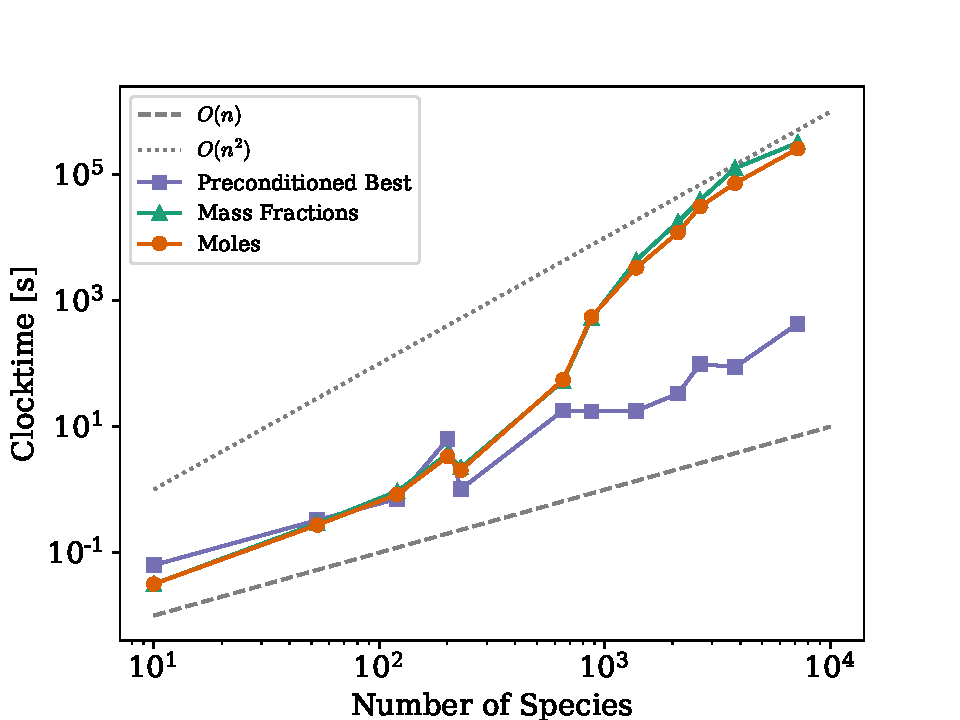
\includegraphics[width=300pt]{figures/Clocktime-Nspecies.pdf}
\vspace{10 pt}
\caption{Engine configuration (top view).}
\label{engine_fig}
\end{figure*}

\sectionOne{Acknowledgements \& References}

The Acknowledgements, Supplementary material (if included), and References section headings are not numbered. The font and spacing are the same as those for regular section headings.

\acknowledgement{Acknowledgments} \addvspace{10pt}

This LaTeX template
